\documentclass[serif,mathserif, 12pt]{beamer}
\usepackage{etex}
\usepackage{amsmath, amsfonts, epsfig, xspace}
\usepackage{algorithm,algorithmic}
\usepackage{pstricks,pst-node}
\usepackage{multimedia}
\usepackage[normal,tight,center]{subfigure}
\setlength{\subfigcapskip}{-.5em}
\usepackage{tkz-euclide}
\usetkzobj{all}
\usepackage{beamerthemesplit}
\usetheme{lankton-keynote}
\usepackage{graphicx,color}
% remove caption of figure
\usepackage[labelformat=empty]{caption}

\usepackage[none]{hyphenat} % hyphenation is ugly in slides
\usepackage{parskip}

\usepackage{relsize} % \smaller to change size

\usepackage{tikz}
\usetikzlibrary{calc}

\usetikzlibrary{arrows}

\newcommand{\TikzDraw}[2][]{
  \begin{tikzpicture}[overlay, remember picture, shift={(current page.center)}, #1]
    #2
  \end{tikzpicture}
}

\newcommand{\gridlines}{
  \TikzDraw{
    \draw[help lines,xstep=.2,ystep=.2,red!20] (current page.south west) grid (current page.north east);
    \draw[help lines,xstep=1,ystep=1,red] (current page.south west) grid (current page.north east);
    \foreach \x in {-15,-14,...,15} {
      \node [anchor=north, red] at (\x,0) {\tiny \x};
      \node [anchor=east,red] at (0,\x) {\tiny \x};
    }
  }
}

\newcommand{\DrawOnImg}[3][]
{
  \begin{tikzpicture}
    \node[anchor=south west,inner sep=0] (image) at (0,0){
      #2
    };
    \begin{scope}[x={(image.south east)},y={(image.north west)}]
      \ifthenelse{\equal{#1}{grid}}
                 {\draw[color=blue, style=dashed] (0,0) grid[xstep=.1, ystep=.1] (1.0001,1.0001);}
                 {}
                 #3
    \end{scope}
  \end{tikzpicture}
}

\usetikzlibrary{matrix}

\newcommand{\BOLD}[1]{\mathbf{#1}}
\newcommand{\BOLDG}[1]{\boldsymbol{#1}}
\newcommand{\PDIF}[2]{\frac{\partial #1}{\partial #2}}
\newcommand{\TODO}[1]{\textcolor{red}{#1}}
\newcommand{\TODOB}[1]{\textcolor{blue}{#1}}
\newcommand{\TODOG}[1]{\textcolor{green!50!black}{#1}}
\newcommand{\argmin}{\operatornamewithlimits{arg\min}}
\DeclareMathOperator{\tr}{tr}
\DeclareMathOperator{\cond}{cond}
\DeclareMathOperator{\ST}{s.t.}
\DeclareMathOperator{\diag}{diag}
\DeclareMathOperator{\Div}{div}

\title[\hspace{2em}\insertframenumber/\inserttotalframenumber]{Eulerian-on-Lagrangian Cloth Simulation}
\date{May 29th, 2018}

\author{Nicholas J. Weidner, Kyle Piddington, \\
  David I.W. Levin, Shinjiro Sueda}

\begin{document}

\maketitle

\begin{frame}
  \frametitle{Challenge}
  \begin{itemize}
  \item The interaction of cloth with sharp geometric features.
    \begin{figure}
      \centering
      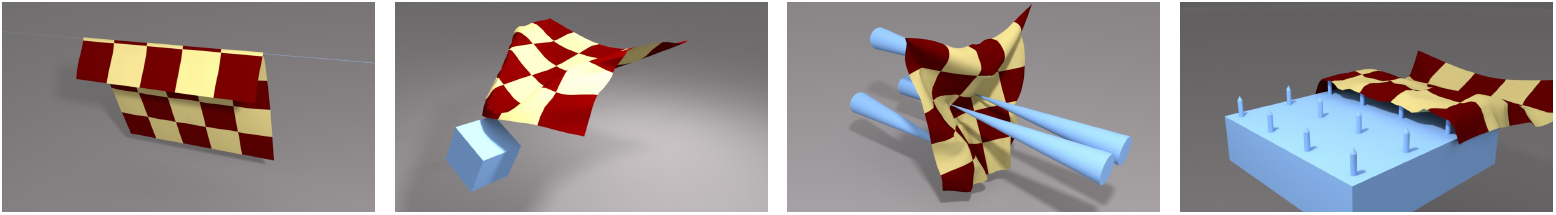
\includegraphics[width=\textwidth]{img/teaser}
    \end{figure}
    \pause
  \item Artifacts of existing Lagrangian methods
    \begin{itemize}
    \item[-] jitter, locking...
    \end{itemize}
  \end{itemize}
  \TikzDraw{
    \node at (2.4, -2.6) {
      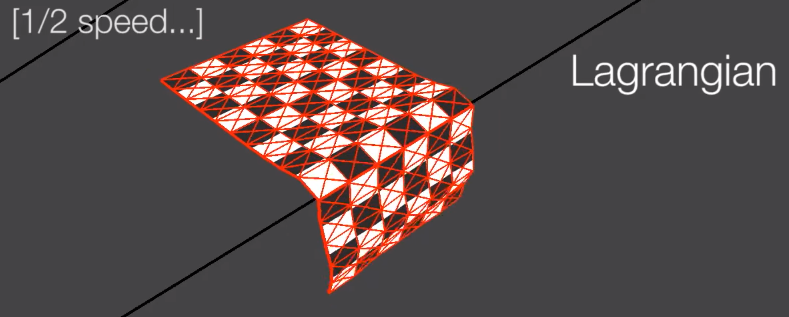
\includegraphics[width=0.5\textwidth]{img/jitter}
    };
  }
\end{frame}

\begin{frame}
  \frametitle{Challenge}
  \begin{figure}
    \centering
    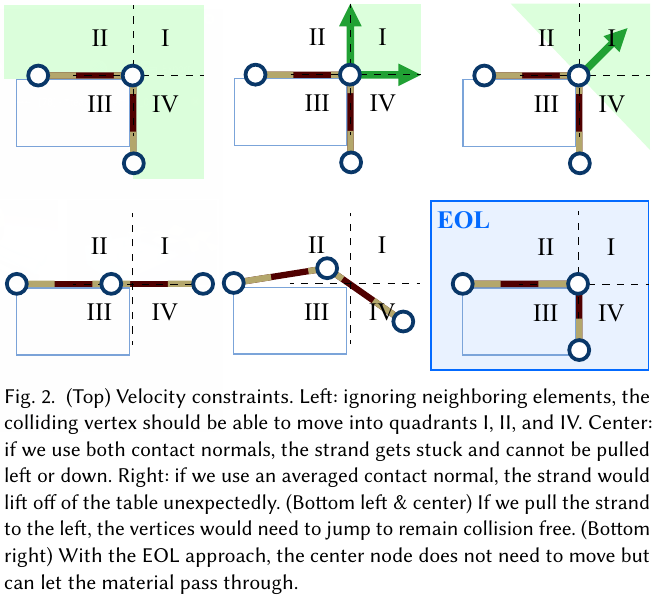
\includegraphics[width=0.8\textwidth]{img/strand}
  \end{figure}
\end{frame}

\begin{frame}
  \frametitle{Idea}
  \begin{itemize}
  \item Eulerian-on-Lagrangian representation
    \begin{itemize}
    \item[-] Moving reference
    \end{itemize}
    \pause
  \item Conformal remeshing algorithm
    \begin{itemize}
    \item[-] DOFs aligned to contact
    \end{itemize}
  \end{itemize}
\end{frame}

\begin{frame}
  \frametitle{Overview}
  \begin{itemize}
  \item From Lagrangian to Eulerian-on-Lagrangian
    \begin{itemize}
    \item[-] Lagrangian vertex: $q_i = x_i \in R^3$
    \item[-] Eulerian-on-Lagrangian (EOL) vertex: $q_i = (x_i, X_i)^T \in R^5$
    \end{itemize}
    \pause
  \item Pipeline
    \begin{figure}
      \centering
      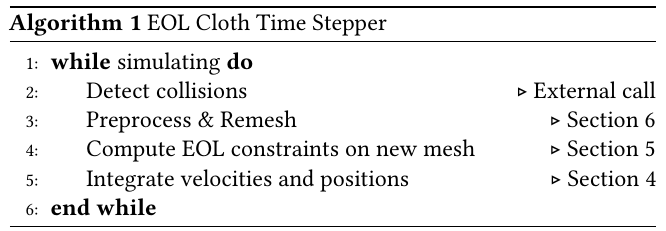
\includegraphics[width=0.8\textwidth]{img/algorithm}
    \end{figure}
  \end{itemize}
\end{frame}

\begin{frame}
  \frametitle{EOL Dynamics}
  \begin{itemize}
  \item World position
    \[
    \begin{split}
    x(X) &= \alpha x_a+\beta x_b + \gamma x_c \\
    \alpha &= \alpha(X, X_a, X_b, X_c)
    \end{split}
    \]
  \item Generalized velocity
    \[
    \begin{split}
      \dot x &= (\alpha \dot x_a+\beta \dot x_b+\gamma \dot x_c)-F(\alpha \dot X_a+\beta \dot X_b+\gamma \dot X_c)\\
      F &= D_xD_X^{-1} = \begin{pmatrix}
        x_b-x_a & x_c-x_a
      \end{pmatrix}
      \begin{pmatrix}
        X_b-X_a & X_c-X_a
      \end{pmatrix}^{-1}
    \end{split}
    \]
  \end{itemize}
\end{frame}

\begin{frame}
  \frametitle{EOL Dynamics}
  \begin{figure}
    \centering
    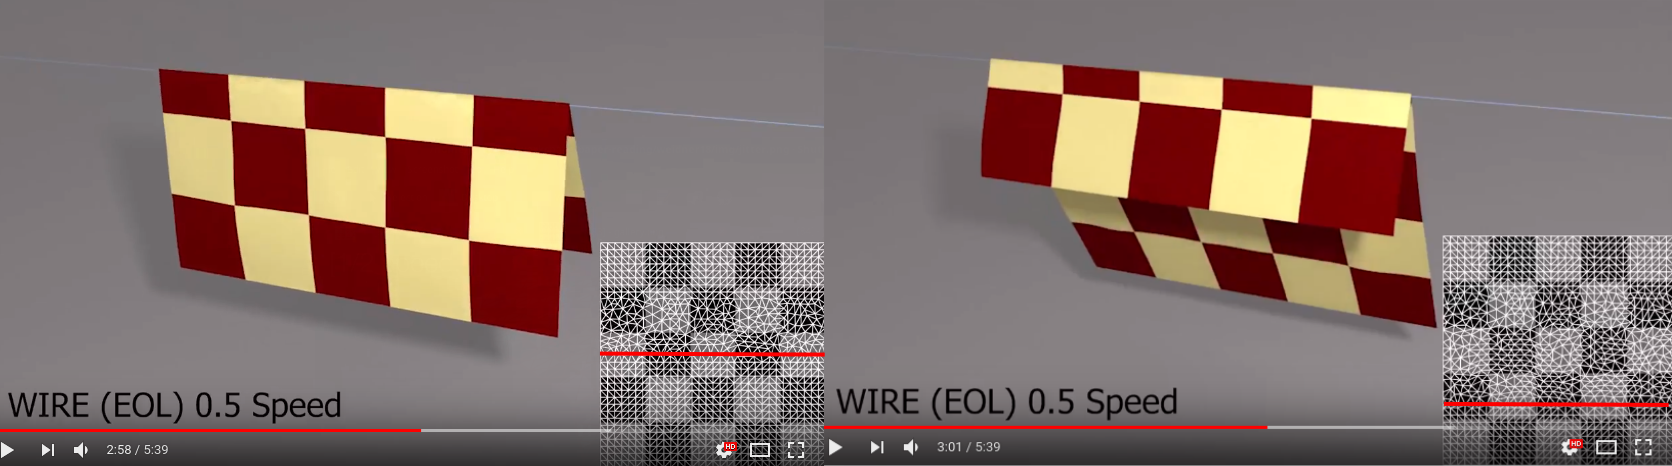
\includegraphics[width=\textwidth]{img/wire_mat_space}
  \end{figure}
\end{frame}

\begin{frame}
  \frametitle{EOL Dynamics}
  \begin{itemize}
  \item Generalized kinetic energy
    \[
    \begin{split}
      T &= \frac{1}{2}\int_A \rho \dot x^T \dot x dA \\
      &=\frac{1}{2}\int_{\alpha=0}^1\int_{\beta}^{1-\alpha} \rho \dot x^T \dot x Ad\beta d\alpha \\
      &= \frac{1}{2} \dot q^T M \dot q
    \end{split}    
    \]
  \item Generalized inertia
    \[
    M = \frac{\rho A}{12}
    \begin{pmatrix}
      2I & I & I & -2F & -F & -F \\
      . & 2I & I & -F & -2F & -F \\
      . & . & 2I & -F & -F & -2F \\
      . & . & . & 2F^TF & F^TF & F^TF \\
      . & . & . & . & 2F^TF & F^TF \\
      . & . & . & . & . & 2F^TF
    \end{pmatrix}
     \]
  \end{itemize}
\end{frame}

\begin{frame}
  \frametitle{EOL Dynamics}
  \begin{itemize}
  \item Generalized forces
    \[
    \begin{pmatrix}
      f^L \\
      f^E
    \end{pmatrix}
    =
    \begin{pmatrix}
      f \\
      -F^Tf
    \end{pmatrix}
    \]
  \item Stiffness matrix
    \[
    \begin{pmatrix}
      K^{LL} & K^{LE} \\
      K^{EL} & K^{EE} 
    \end{pmatrix}
    =
    \begin{pmatrix}
      K & -KF \\
      -F^TK & F^TKF
    \end{pmatrix}
    \]
  \end{itemize}
\end{frame}

\begin{frame}
  \frametitle{EOL Constraints}
  \begin{itemize}
  \item Constraints for Lagrangian cloth
    \begin{itemize}
    \item[-] without conformal remeshing
      \begin{figure}
        \centering
        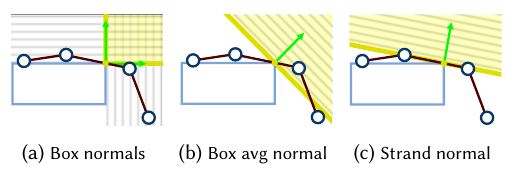
\includegraphics[width=0.5\textwidth]{img/non_conf_lag_cons}
      \end{figure}
    \item[-] with conformal remeshing
      \begin{figure}
        \centering
        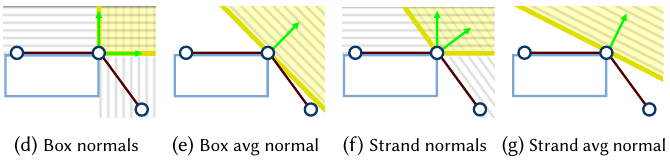
\includegraphics[width=0.6\textwidth]{img/conf_lag_cons}
      \end{figure}
    \end{itemize}
  \end{itemize}
\end{frame}

\begin{frame}
  \frametitle{EOL Constraints}
  \begin{itemize}
  \item Constraints for EOL cloth
    \begin{itemize}
    \item[-] Use Eulerian DOFs to move the cloth around the sharp feature
    \end{itemize}
    \pause
  \item Constraint generation
    \begin{figure}
      \centering
      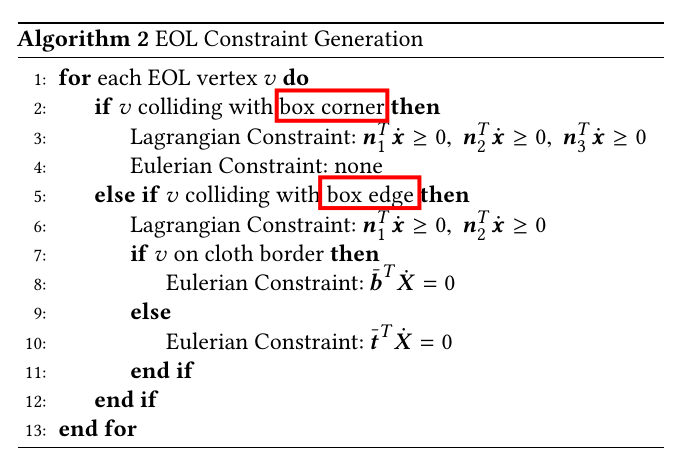
\includegraphics[width=0.7\textwidth]{img/gen_cons}
    \end{figure}
  \end{itemize}
  \TikzDraw{
    \node at (3, 0.5) {
      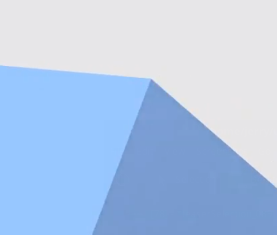
\includegraphics[width=0.15\textwidth]{img/corner}
    };
    \node at (3.5, -2.5) {
      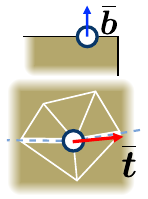
\includegraphics[width=0.15\textwidth]{img/bt}
    };
  }
\end{frame}

\begin{frame}
  \frametitle{Conformal Remeshing}
  \begin{itemize}
  \item \TODO{Preprocessing} + ARCSim
    \begin{itemize}
    \item[-] Collecting conformal vertices and edges (in contact with sharp features)
    \item[-] Insert new conformal vertices untracked
    \item[-] Collapse some vertices
    \item[-] Transfer velocity
    \end{itemize}
  \end{itemize}
  \TikzDraw {
    \visible<2-> {\node at (3, -2) {
      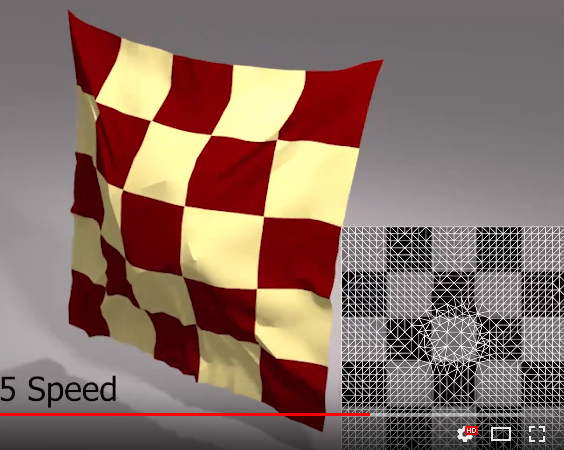
\includegraphics[width=0.4\textwidth]{img/conf_remeshing}
      };
      }
  }
\end{frame}

\begin{frame}
  \TikzDraw {
    \node at (0, 0) {
      \Huge{Results}
    };
  }
\end{frame}

\begin{frame}
  \begin{figure}
    \centering
    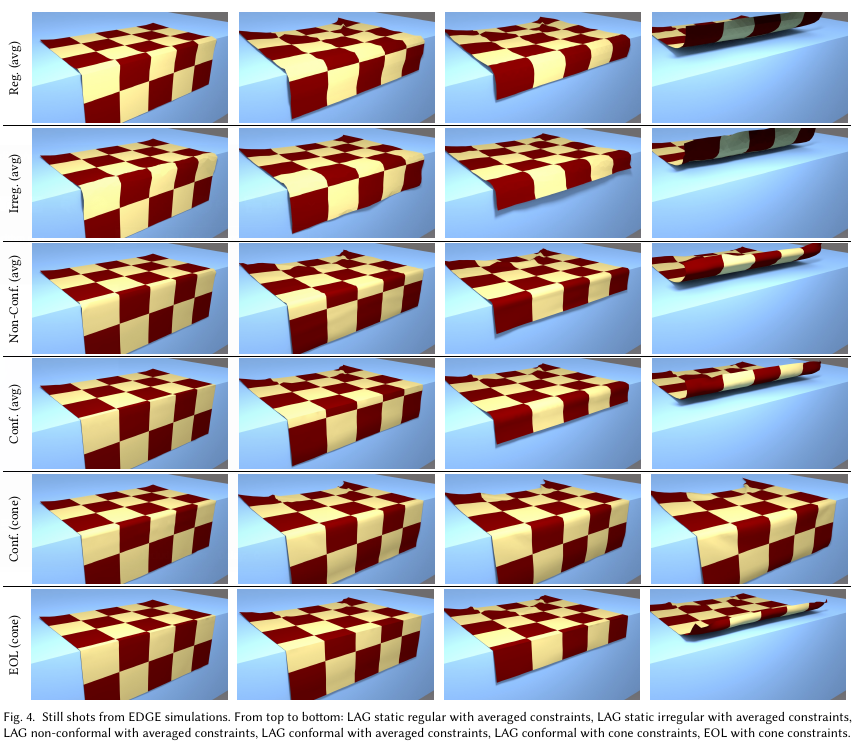
\includegraphics[width=0.9\textwidth]{img/comparison}
  \end{figure}
\end{frame}


\begin{frame}
  \begin{figure}
    \centering
    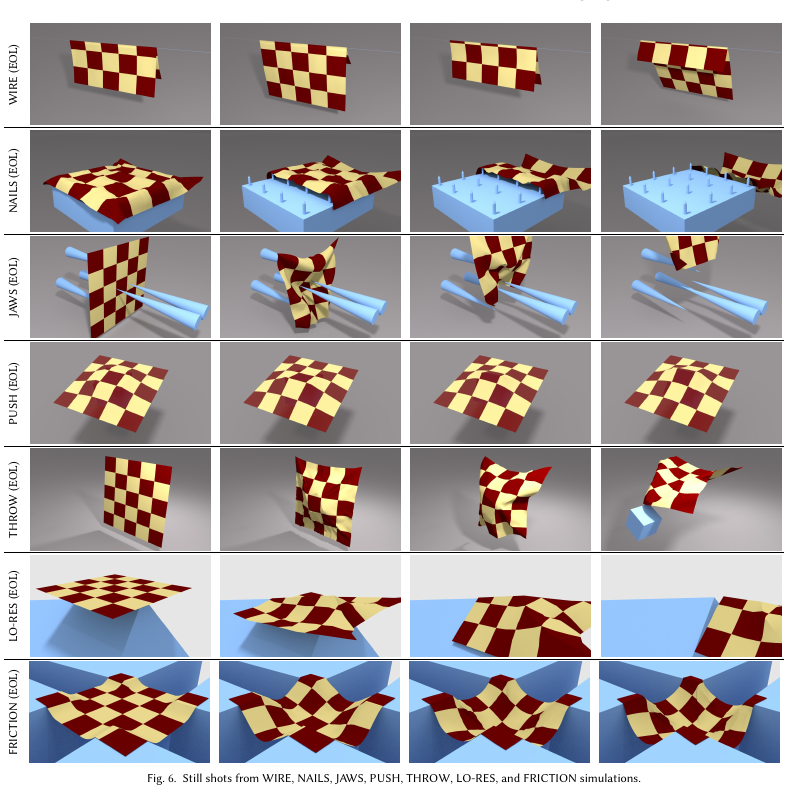
\includegraphics[width=0.8\textwidth]{img/gallery}
  \end{figure}
\end{frame}

\begin{frame} 
  \TikzDraw {
    \node at (0, 0.5) {\Huge{Thanks!}};
  }
  %\gridlines
\end{frame}

\end{document}
